\documentclass[12pt,a4paper]{article}
\usepackage[UTF8]{ctex}
\usepackage{amsmath,amssymb}
\usepackage{listings}
\usepackage{xcolor}
\usepackage{hyperref}
\usepackage{geometry}
\usepackage{graphicx}
\geometry{margin=2.5cm}

\lstdefinestyle{python}{
  language=Python,
  basicstyle=\ttfamily\small,
  keywordstyle=\color{blue}\bfseries,
  commentstyle=\color{gray},
  stringstyle=\color{red},
  showstringspaces=false,
  breaklines=true,
  frame=single,
  backgroundcolor=\color{gray!10}
}

\title{VQE / 变分量子本征求解器}
\author{QuoNic}
\date{}

\begin{document}
\maketitle

\begin{center}
\textbf{Algorithms / 算法} | 难度：高级 | 预计时间：20 分钟
\end{center}

\tableofcontents
\newpage

\section{为什么需要？}

VQE 是量子化学和优化问题的核心算法，是近期量子设备上最有前景的应用之一。

\subsection{经典局限}
\b\begin{itemize}
  \item 经典方法（如 CCSD(T)）对大分子计算成本极高
  \item 精确对角化需要指数级内存
  \item 密度泛函理论（DFT）对强关联体系不准确
\end{itemize}

\subsection{量子优势}
\b\begin{itemize}
  \item VQE 使用量子计算机制备试探态
  \item 经典优化器调整参数最小化能量
  \item 对噪声有鲁棒性，适合近期量子设备
\end{itemize}

\subsection{实际应用}
\b\begin{itemize}
  \item 分子基态能量计算
  \item 药物分子设计
  \item 材料科学（催化剂设计）
  \item 组合优化问题
\end{itemize}

\section{快速上手}

\begin{lstlisting}[style=python]
from quonic.algorithms import vqe
from quonic.chemistry import molecule

# Define H2 molecule
mol = molecule("H2", bond_length=0.74)

# Run VQE
result = vqe(mol, ansatz="uccsd", optimizer="cobyla")
print(f"Ground state energy: {result.energy:.6f} Ha")
\end{lstlisting}

\textbf{预期输出}：
\begin{verbatim}
Ground state energy: -1.137270 Ha
\end{verbatim}

\section{原理详解}

\subsection{电路图}

\begin{center}
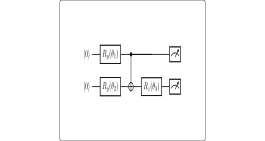
\includegraphics[width=0.6\textwidth]{../../images/vqe_circuit.svg}
\end{center}

\subsection{数学推导}

VQE 基于变分原理：
\begin{equation}
E_0 \leq \langle\psi(\theta)|H|\psi(\theta)\rangle
\end{equation}

其中 $|\psi(\theta)\rangle$ 是参数化量子态（ansatz），$H$ 是哈密顿量。

\textbf{算法步骤}：
\begin{enumerate}
  \item 在量子计算机上制备 $|\psi(\theta)\rangle$
  \item 测量哈密顿量的期望值 $\langle H \rangle$
  \item 经典优化器更新参数 $\theta$
  \item 重复直到收敛
\end{enumerate}

\subsection{几何解释}

VQE 在参数空间中寻找能量最小值。量子计算机负责制备态和测量，经典优化器负责更新参数。

\section{代码详解}

\begin{lstlisting}[style=python]
from quonic.algorithms import vqe
from quonic.chemistry import molecule

# Define molecule
mol = molecule("H2", bond_length=0.74)

# vqe(molecule, ansatz, optimizer)
# molecule: molecular system
# ansatz: parameterized circuit (UCCSD, hardware-efficient)
# optimizer: classical optimizer (COBYLA, L-BFGS-B, SPSA)
result = vqe(mol, ansatz="uccsd", optimizer="cobyla")

# result.energy: ground state energy
# result.params: optimized parameters
# result.history: optimization history
print(f"Energy: {result.energy:.6f} Ha")
\end{lstlisting}

\section{进阶用法}

\subsection{场景 1：不同分子}

\begin{lstlisting}[style=python]
# Different molecules
mol_h2o = molecule("H2O", bond_length=0.96)
mol_lih = molecule("LiH", bond_length=1.6)

result_h2o = vqe(mol_h2o, ansatz="uccsd")
result_lih = vqe(mol_lih, ansatz="uccsd")
\end{lstlisting}

\subsection{场景 2：不同 ansatz}

\begin{lstlisting}[style=python]
# Hardware-efficient ansatz
result = vqe(mol, ansatz="hardware_efficient", depth=3)

# UCCSD ansatz
result = vqe(mol, ansatz="uccsd")
\end{lstlisting}

\subsection{场景 3：带噪声的 VQE}

\begin{lstlisting}[style=python]
# VQE with noise mitigation
result = vqe(mol, ansatz="uccsd", noise_mitigation=True)
\end{lstlisting}

\section{适用场景}

\subsection{量子化学}

VQE 是量子化学计算的核心算法，用于计算分子基态能量。

\subsection{材料科学}

VQE 可以用于设计新型催化剂和材料。

\subsection{组合优化}

VQE 可以用于解决组合优化问题，如 MaxCut。

\section{常见问题}

\subsection{VQE 和 QAOA 有什么区别？}

VQE 用于量子化学（连续优化），QAOA 用于组合优化（离散优化）。

\subsection{VQE 的精度如何？}

VQE 的精度取决于 ansatz 的表达能力和优化器的性能。UCCSD ansatz 通常能达到化学精度（1 kcal/mol）。

\subsection{VQE 需要多少量子比特？}

VQE 需要的量子比特数取决于分子的大小。H2 需要 4 个量子比特，H2O 需要 14 个。

\section{学习路径}

\subsection{前置知识}
\b\begin{itemize}
  \item 量子化学基础
  \item 变分原理
  \item 参数化量子电路
\end{itemize}

\subsection{继续学习}
\b\begin{itemize}
  \item QAOA（组合优化）
  \item 量子化学模拟
  \item 量子机器学习
\end{itemize}

\section{完整示例代码}

\subsection{示例 1：基本 VQE}

\begin{lstlisting}[style=python]
from quonic.algorithms import vqe
from quonic.chemistry import molecule

mol = molecule("H2", bond_length=0.74)
result = vqe(mol, ansatz="uccsd", optimizer="cobyla")
print(f"Energy: {result.energy:.6f} Ha")
\end{lstlisting}

\

\section{下载}

\begin{itemize}
  \item [vqe.py](https://github.com/ChrisLee0721/QuoNic/blob/main/examples/vqe/vqe.py)
\end{itemize}

\end{document}
